% Author: Izaak Neutelings (September 2021)
% Inspiration:
%   https://www.asimovinstitute.org/neural-network-zoo/
%   https://www.youtube.com/watch?v=aircAruvnKk&list=PLZHQObOWTQDNU6R1_67000Dx_ZCJB-3pi&index=1
\documentclass[border=3pt,tikz]{standalone}
\usepackage{amsmath} % for aligned
%\usepackage{amssymb} % for \mathbb
\usepackage{tikz}
%\usepackage{etoolbox} % for \ifthen
\usepackage{listofitems} % for \readlist to create arrays
\usetikzlibrary{arrows.meta} % for arrow size
\usepackage[outline]{contour} % glow around text
\contourlength{1.4pt}

\tikzset{>=latex} % for LaTeX arrow head
\usepackage{xcolor}
\colorlet{myred}{red!80!black}
\colorlet{myblue}{blue!80!black}
\colorlet{mygreen}{green!60!black}
\colorlet{myorange}{orange!70!red!60!black}
\colorlet{mydarkred}{red!30!black}
\colorlet{mydarkblue}{blue!40!black}
\colorlet{mydarkgreen}{green!30!black}
\tikzstyle{node}=[thick,circle,draw=myblue,minimum size=22,inner sep=0.5,outer sep=0.6]
\tikzstyle{node in}=[node,green!20!black,draw=mygreen!30!black,fill=mygreen!25]
\tikzstyle{node hidden}=[node,blue!20!black,draw=myblue!30!black,fill=myblue!20]
\tikzstyle{node convol}=[node,orange!20!black,draw=myorange!30!black,fill=myorange!20]
\tikzstyle{node out}=[node,red!20!black,draw=myred!30!black,fill=myred!20]
\tikzstyle{connect}=[thick,mydarkblue] %,line cap=round
\tikzstyle{connect arrow}=[-{Latex[length=4,width=3.5]},thick,mydarkblue,shorten <=0.5,shorten >=1]
\tikzset{ % node styles, numbered for easy mapping with \nstyle
  node 1/.style={node in},
  node 2/.style={node hidden},
  node 3/.style={node out},
}
\def\nstyle{int(\lay<\Nnodlen?min(2,\lay):3)} % map layer number onto 1, 2, or 3
\begin{document}

% NEURAL NETWORK activation
% https://www.youtube.com/watch?v=aircAruvnKk&list=PLZHQObOWTQDNU6R1_67000Dx_ZCJB-3pi&index=1
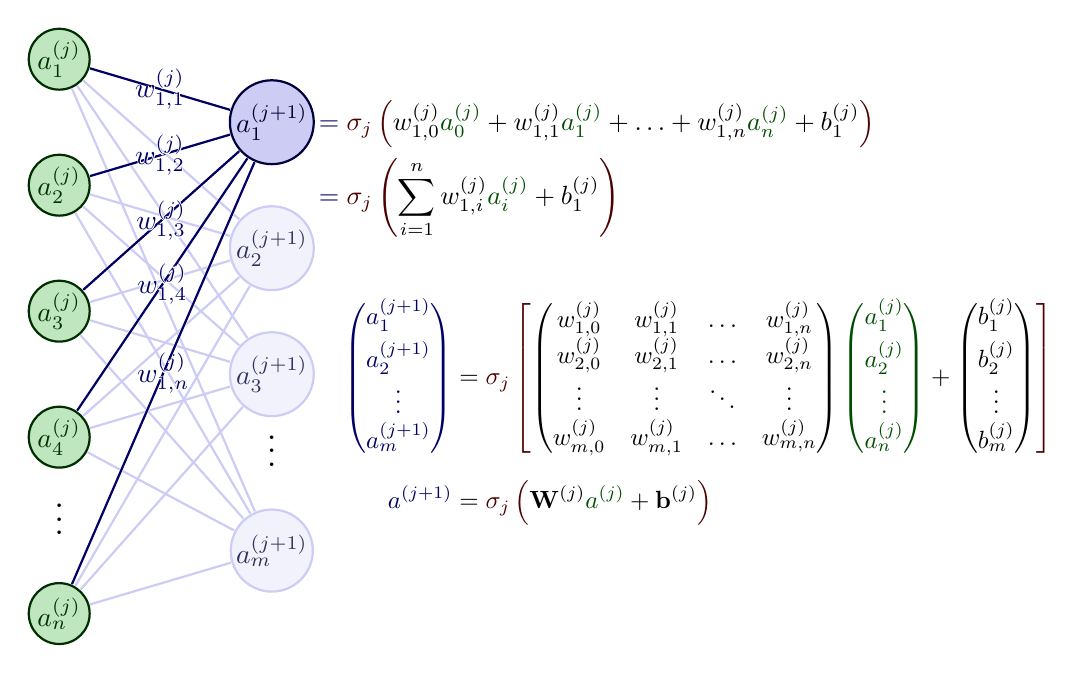
\begin{tikzpicture}[x=2.7cm,y=1.6cm]
    \message{^^JNeural network activation}
    \def\NI{5} % number of nodes in input layers
    \def\NO{4} % number of nodes in output layers
    \def\yshift{0.4} % shift last node for dots

    % INPUT LAYER
    \foreach \i [evaluate={\c=int(\i==\NI); \y=\NI/2-\i-\c*\yshift; \index=(\i<\NI?int(\i):"n");}]
    in {1,...,\NI}{ % loop over nodes
            \node[node in,outer sep=0.6] (NI-\i) at (0,\y) {$a_{\index}^{(j)}$};
        }

    % OUTPUT LAYER
    \foreach \i [evaluate={\c=int(\i==\NO); \y=\NO/2-\i-\c*\yshift; \index=(\i<\NO?int(\i):"m");}]
    in {\NO,...,1}{ % loop over nodes
            \ifnum\i=1 % high-lighted node
                \node[node hidden]
                (NO-\i) at (1,\y) {$a_{\index}^{(j+1)}$};
                \foreach \j [evaluate={\index=(\j<\NI?int(\j):"n");}] in {1,...,\NI}{ % loop over nodes in previous layer
                        \draw[connect,white,line width=1.2] (NI-\j) -- (NO-\i);
                        \draw[connect] (NI-\j) -- (NO-\i)
                        node[pos=0.50] {\contour{white}{$w_{1,\index}^{(j)}$}};
                    }
            \else % other light-colored nodes
                \node[node,blue!20!black!80,draw=myblue!20,fill=myblue!5]
                (NO-\i) at (1,\y) {$a_{\index}^{(j + 1)}$};
                \foreach \j in {1,...,\NI}{ % loop over nodes in previous layer
                        %\draw[connect,white,line width=1.2] (NI-\j) -- (NO-\i);
                        \draw[connect,myblue!20] (NI-\j) -- (NO-\i);
                    }
            \fi
        }

    % DOTS
    \path (NI-\NI) --++ (0,1+\yshift) node[midway,scale=1.2] {$\vdots$};
    \path (NO-\NO) --++ (0,1+\yshift) node[midway,scale=1.2] {$\vdots$};

    % EQUATIONS
    \def\agr#1{{\color{mydarkgreen}a_{#1}^{(j)}}}
    \node[below=17,right=11,mydarkblue,scale=0.95] at (NO-1)
    {$\begin{aligned} %\underset{\text{bias}}{b_1}
                 & = \color{mydarkred}\sigma_j\left( \color{black}
                w_{1,0}^{(j)}\agr{0} + w_{1,1}^{(j)}\agr{1} + \ldots + w_{1,n}^{(j)}\agr{n} + b_1^{(j)}
                \color{mydarkred}\right)                           \\
                 & = \color{mydarkred}\sigma_j\left( \color{black}
                \sum_{i=1}^{n} w_{1,i}^{(j)}\agr{i} + b_1^{(j)}
                \color{mydarkred}\right)
            \end{aligned}$};
    \node[right,scale=0.9] at (1.3,-1.3)
    {$\begin{aligned}
                {\color{mydarkblue}
                    \begin{pmatrix}
                        a_{1}^{(j + 1)} \\[0.3em]
                        a_{2}^{(j + 1)} \\
                        \vdots          \\
                        a_{m}^{(j + 1)}
                    \end{pmatrix}}
                 & =
                \color{mydarkred}\sigma_j\left[ \color{black}
                \begin{pmatrix}
                    w_{1,0}^{(j)} & w_{1,1}^{(j)} & \ldots & w_{1,n}^{(j)} \\
                    w_{2,0}^{(j)} & w_{2,1}^{(j)} & \ldots & w_{2,n}^{(j)} \\
                    \vdots        & \vdots        & \ddots & \vdots        \\
                    w_{m,0}^{(j)} & w_{m,1}^{(j)} & \ldots & w_{m,n}^{(j)}
                \end{pmatrix}
                {\color{mydarkgreen}
                \begin{pmatrix}
                    a_{1}^{(j)} \\[0.3em]
                    a_{2}^{(j)} \\
                    \vdots      \\
                    a_{n}^{(j)}
                \end{pmatrix}}
                +
                \begin{pmatrix}
                    b_{1}^{(j)} \\[0.3em]
                    b_{2}^{(j)} \\
                    \vdots      \\
                    b_{m}^{(j)}
                \end{pmatrix}
                \color{mydarkred}\right]                           \\[0.5em]
                {\color{mydarkblue}a^{(j+1)}}
                 & = \color{mydarkred}\sigma_j\left( \color{black}
                \mathbf{W}^{(j)} {\color{mydarkgreen}a^{(j)}}+\mathbf{b}^{(j)}
                \color{mydarkred}\right)
                %\color{black},\quad \mathbf{W}^{(0)} \in \mathbb{R}^{m\times n}
            \end{aligned}$};

\end{tikzpicture}


\end{document}